\section{Рабочий проект}
\subsection{Спецификация классов фреймворка}

Класс Framework инициализирует фреймфорк. Запускает GDI+. Запускает или останавливает работу. (таблица \ref{framework_m:table}).

\renewcommand{\arraystretch}{0.8} % уменьшение расстояний до сетки таблицы
\begin{xltabular}{\textwidth}{|X|>{\setlength{\baselineskip}{0.7\baselineskip}}p{4.85cm}|>{\setlength{\baselineskip}{0.7\baselineskip}}p{4.85cm}|}
	\caption{Спецификация методов класса Framework\label{framework_m:table}}\\
	\hline \centrow \setlength{\baselineskip}{0.7\baselineskip} Название & \centrow Метод дрступа & \centrow Описание \\
	\hline \centrow 1 & \centrow 2 & \centrow 3 \\ \hline
	\endfirsthead
	\continuecaption{Продолжение таблицы \ref{framework_m:table}}
	\hline \centrow 1 & \centrow 2 & \centrow 3 \\ \hline
	\finishhead
	init & public & Запуск GDI+ \\ \hline
	run & public & Запускает приложение \\ \hline
	stop & public & Останавливает работу приложения
\end{xltabular}
\renewcommand{\arraystretch}{1.0} % восстановление сетки

Класс Window создает окна для приложения. Принимает системные события и обеспечивает их рассылку подписчикам. Так же окно дает команду на перерисовку своих компонентов и предоставляет им свой graphic. Кроме этого, окно управляет фокусом ввода, может сделать модальность и отправить подписанному пользователю или в систему событие. (таблица \ref{window_m:table}).

\renewcommand{\arraystretch}{0.8} % уменьшение расстояний до сетки таблицы
\begin{xltabular}{\textwidth}{|X|>{\setlength{\baselineskip}{0.7\baselineskip}}p{4.85cm}|>{\setlength{\baselineskip}{0.7\baselineskip}}p{4.85cm}|}
	\caption{Спецификация методов класса Window\label{window_m:table}}\\
	\hline \centrow \setlength{\baselineskip}{0.7\baselineskip} Название & \centrow Метод дрступа & \centrow Описание \\
	\hline \centrow 1 & \centrow 2 & \centrow 3 \\ \hline
	\endfirsthead
	\continuecaption{Продолжение таблицы \ref{window_m:table}}
	\hline \centrow 1 & \centrow 2 & \centrow 3 \\ \hline
	\finishhead
	init & public & Создание окна \\ \hline
	destroy & public & Уничтожение  окна \\ \hline
	add{\_}control & public & Добавление контрола \\ \hline
	remove{\_}control & public & Удаление контрола \\ \hline
	bring{\_}to{\_}front, move{\_}to{\_}back & public & Изменеие порядка слоев элементов \\ \hline
	set{\_}position & public & Изменеие позиции окна \\ \hline
	position & public & Возвращение позиции окна \\ \hline
	set{\_}parent & public & Установление родительского окна \\ \hline
	parent & public & Возвращение родительского окна \\ \hline
	clear{\_}parent & public & Очищение свойства родительского окна \\ \hline
	update{\_}theme & public & Обновление темы \\ \hline
	redraw & public & Перерисовывает часть окна. Вызывается компонентом окна. \\ \hline
	subscribe & public & Подписка на события \\ \hline
	unsubscribe & public & Отписка от событий \\ \hline
	emit{\_}event & public & Посылает сообщение через системный шедулер сообщений \\ \hline
	set{\_}caption & public & Изменяет название окна \\ \hline
	set{\_}style & public & Изменяет стиль окна \\ \hline
	set{\_}min{\_}size & public & Изменяет минимальный размер окна \\ \hline
	switch{\_}lang & public & Изменяет язык  \\ \hline
	switch{\_}theme & public & Изменяет тему  \\ \hline
	pin & public & Прикрепляет окно \\ \hline
	minimize & public & Сворачивает окно \\ \hline
	expand & public & Расширяет окно \\ \hline
	normal & public & Возвращает окно в исходное состояние \\ \hline
	state & public & Изменяет состояние окна \\ \hline
	disable{\_}draw, enable{\_}draw& public & Отключает/Включает рисование для повышения производительности при выполнении массовых операций \\ \hline
	set{\_}focused & public & Делает компонент окна сфокусированным \\ \hline
	set{\_}control{\_}callback & public & Привязывает событие к компоненту \\ \hline
	set{\_}default{\_}push{\_}control & public & Нажатие кнопки по клавише Enter \\ \hline
	receive{\_}control{\_}events & private & Принимает события от компонентов \\ \hline
	send{\_}event{\_}to{\_}control & private & Посылает событие компоненту \\ \hline
	send{\_}mouse{\_}event & private & Посылает событие мыши \\ \hline
	check{\_}control{\_}here & private & Проверяет компонент на месте клика \\ \hline
	change{\_}focus & private & Изменяет фокус \\ \hline
	get{\_}focused & private & Возвращает сфокусированый элемент \\ \hline
	start{\_}docking, end{\_}docking & private & Включает/отключает привязку к окну \\ \hline
	draw{\_}border & private & Рисукет границы графического контекста \\ \hline
	send{\_}system & private & Отправить системное сообщение
\end{xltabular}
\renewcommand{\arraystretch}{1.0} % восстановление сетки

Класс Control - это любой визуальный элемент для взаимодействия с пользователем - кнопка, поле ввода, список, меню и т.д. Control знает, как обрабатывать события, поступающие от Window, хранит свои состояния и рисует себя на графическом контексте, который предоставляется содержащим его окном. (таблица \ref{control_m:table}).

\renewcommand{\arraystretch}{0.8} % уменьшение расстояний до сетки таблицы
\begin{xltabular}{\textwidth}{|X|>{\setlength{\baselineskip}{0.7\baselineskip}}p{4.85cm}|>{\setlength{\baselineskip}{0.7\baselineskip}}p{4.85cm}|}
	\caption{Спецификация методов класса Сontrol\label{control_m:table}}\\
	\hline \centrow \setlength{\baselineskip}{0.7\baselineskip} Название & \centrow Метод дрступа & \centrow Описание \\
	\hline \centrow 1 & \centrow 2 & \centrow 3 \\ \hline
	\endfirsthead
	\continuecaption{Продолжение таблицы \ref{control_m:table}}
	\hline \centrow 1 & \centrow 2 & \centrow 3 \\ \hline
	\finishhead
	draw & public & Рисует компонент. Вызывается окном. \\ \hline
	set{\_}position & public & Изменяет положение контрола на окне. Координаты задаются в пикселях относительно левого верхнего угла родительского окна.  \\ \hline
	position & public & Возвращает положение контрола относительно окна \\ \hline
	set{\_}parent & public & Позволяет контролу получить указатель на свое родительское окно \\ \hline
	parent & public & Возвращает указатель на родительское окно \\ \hline
	clear{\_}parent & public & Очищает указатель на родительское окно контрола \\ \hline
	topmost & public & Сообщает родительскому окну, нужно ли рисовать контрол поверх всех остальных контролов \\ \hline
	update{\_}theme & public & Изменяет визуальную тему контрола \\ \hline
	show,hide,showed & public & Методы управления видимостью \\ \hline
	enable,disable,enabled & public & Методы управления включенностью \\ \hline
	focused,focusing & public & Клавиатурный фокус ввода \\ \hline
	get{\_}error & public & Возвращает структуру, содержащую подробности последней ошибки
\end{xltabular}
\renewcommand{\arraystretch}{1.0} % восстановление сетки

Класс Image создает изображение на экране. (таблица \ref{image_m:table}).

\renewcommand{\arraystretch}{0.8} % уменьшение расстояний до сетки таблицы
\begin{xltabular}{\textwidth}{|X|>{\setlength{\baselineskip}{0.7\baselineskip}}p{4.85cm}|>{\setlength{\baselineskip}{0.7\baselineskip}}p{4.85cm}|}
	\caption{Спецификация методов класса Image\label{image_m:table}}\\
	\hline \centrow \setlength{\baselineskip}{0.7\baselineskip} Название & \centrow Метод дрступа & \centrow Описание \\
	\hline \centrow 1 & \centrow 2 & \centrow 3 \\ \hline
	\endfirsthead
	\continuecaption{Продолжение таблицы \ref{image_m:table}}
	\hline \centrow 1 & \centrow 2 & \centrow 3 \\ \hline
	\finishhead
	image & public & Создает изображение \\ \hline
	change{\_}image & public & Изменяет изображение \\ \hline
	width, height & public & Возвращает ширину/высоту изображения \\ \hline
	draw & public & Рисует изображение. Вызывается окном. \\ \hline
	set{\_}position & public & Изменяет положение контрола на окне. Координаты задаются в пикселях относительно левого верхнего угла родительского окна.  \\ \hline
	position & public & Возвращает положение контрола относительно окна \\ \hline
	set{\_}parent & public & Позволяет контролу получить указатель на свое родительское окно \\ \hline
	parent & public & Возвращает указатель на родительское окно \\ \hline
	clear{\_}parent & public & Очищает указатель на родительское окно контрола \\ \hline
	topmost & public & Сообщает родительскому окну, нужно ли рисовать контрол поверх всех остальных контролов \\ \hline
	update{\_}theme & public & Изменяет визуальную тему контрола \\ \hline
	show,hide,showed & public & Методы управления видимостью \\ \hline
	enable,disable,enabled & public & Методы управления включенностью \\ \hline
	focused,focusing & public & Клавиатурный фокус ввода \\ \hline
	get{\_}error & public & Возвращает структуру, содержащую подробности последней ошибки
\end{xltabular}
\renewcommand{\arraystretch}{1.0} % восстановление сетки

Класс Button - это любая кнопка для взаимодействия с пользователем. Кнопка знает, как обрабатывать события, поступающие от Window, хранит свои состояния и рисует себя на графическом контексте, который предоставляется содержащим его окном. (таблица \ref{button_m:table}).

\renewcommand{\arraystretch}{0.8} % уменьшение расстояний до сетки таблицы
\begin{xltabular}{\textwidth}{|X|>{\setlength{\baselineskip}{0.7\baselineskip}}p{4.85cm}|>{\setlength{\baselineskip}{0.7\baselineskip}}p{4.85cm}|}
	\caption{Спецификация методов класса Button\label{button_m:table}}\\
	\hline \centrow \setlength{\baselineskip}{0.7\baselineskip} Название & \centrow Метод дрступа & \centrow Описание \\
	\hline \centrow 1 & \centrow 2 & \centrow 3 \\ \hline
	\endfirsthead
	\continuecaption{Продолжение таблицы \ref{button_m:table}}
	\hline \centrow 1 & \centrow 2 & \centrow 3 \\ \hline
	\finishhead
	button & public & Функция создания кнопки. \\ \hline
	draw & public & Рисует кнопку. \\ \hline
	set{\_}position & public & Изменяет положение контрола на окне. Координаты задаются в пикселях относительно левого верхнего угла родительского окна.  \\ \hline
	position & public & Возвращает положение контрола относительно окна \\ \hline
	set{\_}parent & public & Позволяет контролу получить указатель на свое родительское окно \\ \hline
	parent & public & Возвращает указатель на родительское окно \\ \hline
	clear{\_}parent & public & Очищает указатель на родительское окно контрола \\ \hline
	topmost & public & Сообщает родительскому окну, нужно ли рисовать контрол поверх всех остальных контролов \\ \hline
	update{\_}theme & public & Изменяет визуальную тему контрола \\ \hline
	show,hide,showed & public & Методы управления видимостью \\ \hline
	enable,disable,enabled & public & Методы управления включенностью \\ \hline
	focused,focusing & public & Клавиатурный фокус ввода \\ \hline
	get{\_}error & public & Возвращает структуру, содержащую подробности последней ошибки\\ \hline
	update{\_}err & private & Обновляет структуру ошибки\\ \hline
	set{\_}caption & private & Устанавливает надпись на кнопке\\ \hline
	set{\_}button{\_}view & private & Изменяет вид кнопки\\ \hline
	set{\_}image & private & Устанавливает изображение на кнопку\\ \hline
	enable{\_}focusing & private & Включает фокус\\ \hline
	disable{\_}focusing & private & Отключает фокус\\ \hline
	turn & private & Включает кнопку\\ \hline
	turned & private & Возвращает флаг включения кнопки\\ \hline
	set{\_}callback & private & Устанавливает функионал кнопки \\ \hline
	receive{\_}event & private & Получение события \\ \hline
	redraw & private & Перерисовывает кнопку
\end{xltabular}  
\renewcommand{\arraystretch}{1.0} % восстановление сетки

Класс Graphic предоставляет интерфейс к системным методам рисования. В настоящий момент, реализовано рисование на Windows GDI/GDI+. (таблица \ref{graphic:table}).

\renewcommand{\arraystretch}{0.8} % уменьшение расстояний до сетки таблицы
\begin{xltabular}{\textwidth}{|X|>{\setlength{\baselineskip}{0.7\baselineskip}}p{4.85cm}|>{\setlength{\baselineskip}{0.7\baselineskip}}p{4.85cm}|}
	\caption{Спецификация методов класса Graphic\label{graphic:table}}\\
	\hline \centrow \setlength{\baselineskip}{0.7\baselineskip} Название & \centrow Метод дрступа & \centrow Описание \\
	\hline \centrow 1 & \centrow 2 & \centrow 3 \\ \hline
	\endfirsthead
	\continuecaption{Продолжение таблицы \ref{graphic:table}}
	\hline \centrow 1 & \centrow 2 & \centrow 3 \\ \hline
	\finishhead
	init & public & Инициализация \\ \hline
	release & public & Деинициализации  \\ \hline
	set{\_}background{\_}color & public & Устанавливает цвет фона \\ \hline
	clear & public & Заливает холст \\ \hline
	flush & public & Отрисовка области на системный графический контекст \\ \hline
	draw{\_}pixel{\_} & public & Рисует точку \\ \hline
	draw{\_}line & public & Рисует линию \\ \hline
	measure{\_}text & public & Измеряет размер текста с выбранным шрифтом \\ \hline
	draw{\_}text & public & Рисует текст \\ \hline
	draw{\_}rect & public & Рисует прямоугольник \\ \hline
	draw{\_}buffer & public & Рисует буфер RGB32 \\ \hline
	draw{\_}graphic & public & Рисует содержимое другого графика
\end{xltabular}
\renewcommand{\arraystretch}{1.0} % восстановление сетки

Класс Locale нужен для смены языка программы. Он загружает текстовые константы, меняет текущий язык, а также загружает json-файл для быстрой настройки. (таблица \ref{locale_m:table}).

\renewcommand{\arraystretch}{0.8} % уменьшение расстояний до сетки таблицы
\begin{xltabular}{\textwidth}{|X|>{\setlength{\baselineskip}{0.7\baselineskip}}p{4.85cm}|>{\setlength{\baselineskip}{0.7\baselineskip}}p{4.85cm}|}
	\caption{Спецификация методов класса Locale\label{locale_m:table}}\\
	\hline \centrow \setlength{\baselineskip}{0.7\baselineskip} Название & \centrow Метод дрступа & \centrow Описание \\
	\hline \centrow 1 & \centrow 2 & \centrow 3 \\ \hline
	\endfirsthead
	\continuecaption{Продолжение таблицы \ref{locale_m:table}}
	\hline \centrow 1 & \centrow 2 & \centrow 3 \\ \hline
	\finishhead
	get{\_}type() & public & Возвращает код языка \\ \hline
	get{\_}name & public & Возвращает название перевода \\ \hline
	set & public & Меняет текущий язык \\ \hline
	get & public & Возвращает данные перевода \\ \hline
	load{\_}resource & public & Загружает ресурсы перевода \\ \hline
	load{\_}json & public & Загружает json-файл перевода \\ \hline
	load{\_}locale & public & Загружает строки перевода
\end{xltabular}
\renewcommand{\arraystretch}{1.0} % восстановление сетки

Класс Theme нужен для изменение цветовых акцентов окна. Он позволяет менять цвета, шрифты, изображение, а также загружать json-файлы для быстрой настройки. (таблица \ref{theme_m:table}).

\renewcommand{\arraystretch}{0.8} % уменьшение расстояний до сетки таблицы
\begin{xltabular}{\textwidth}{|X|>{\setlength{\baselineskip}{0.7\baselineskip}}p{4.85cm}|>{\setlength{\baselineskip}{0.7\baselineskip}}p{4.85cm}|}
	\caption{Спецификация методов класса Theme\label{theme_m:table}}\\
	\hline \centrow \setlength{\baselineskip}{0.7\baselineskip} Название & \centrow Метод дрступа & \centrow Описание \\
	\hline \centrow 1 & \centrow 2 & \centrow 3 \\ \hline
	\endfirsthead
	\continuecaption{Продолжение таблицы \ref{theme_m:table}}
	\hline \centrow 1 & \centrow 2 & \centrow 3 \\ \hline
	\finishhead
	get{\_}name & public & Возвращает название темы \\ \hline
	set{\_}color & public & Меняет цвет \\ \hline
	get{\_}color & public & Возвращает цвет \\ \hline
	set{\_}string & public & Меняет текст \\ \hline
	get{\_}string & public & Возвращает текст \\ \hline
	set{\_}font & public & Меняет шрифт \\ \hline
	get{\_}font & public & Возвращает шрифт \\ \hline
	set{\_}image & public & Меняет изображение \\ \hline
	get{\_}image & public & Возвращает изображение \\ \hline
	load{\_}resource & public & Загружает ресурсы темы \\ \hline
	load{\_}json & public & Загружает json-файл темы \\ \hline
	load{\_}theme & public & Загружает данные темы
\end{xltabular}
\renewcommand{\arraystretch}{1.0} % восстановление сетки

Класс Config меняет значения регистра. Работает с определенными типами данных. (таблица \ref{config_m:table})

\renewcommand{\arraystretch}{0.8} % уменьшение расстояний до сетки таблицы
\begin{xltabular}{\textwidth}{|X|>{\setlength{\baselineskip}{0.7\baselineskip}}p{4.85cm}|>{\setlength{\baselineskip}{0.7\baselineskip}}p{4.85cm}|}
	\caption{Спецификация методов класса Config\label{config_m:table}}\\
	\hline \centrow \setlength{\baselineskip}{0.7\baselineskip} Название & \centrow Метод дрступа & \centrow Описание \\
	\hline \centrow 1 & \centrow 2 & \centrow 3 \\ \hline
	\endfirsthead
	\continuecaption{Продолжение таблицы \ref{config_m:table}}
	\hline \centrow 1 & \centrow 2 & \centrow 3 \\ \hline
	\finishhead
	get{\_}int & public & Возвращает целое число \\ \hline
	set{\_}int & public & Меняет целое число \\ \hline
	get{\_}int64 & public & Возвращает большое число \\ \hline
	set{\_}int64 & public & Меняет большое число \\ \hline
	get{\_}string & public & Возвращает строку \\ \hline
	set{\_}string & public & Меняет строку \\ \hline
	delete{\_}value & public & Удаляет значение из регистра \\ \hline
	delete{\_}key & public & Удаляет ключ из регистра
\end{xltabular}
\renewcommand{\arraystretch}{1.0} % восстановление сетки

Класс Error выводит сообщения об ошибках. (таблица \ref{error_m:table})

\renewcommand{\arraystretch}{0.8} % уменьшение расстояний до сетки таблицы
\begin{xltabular}{\textwidth}{|X|>{\setlength{\baselineskip}{0.7\baselineskip}}p{4.85cm}|>{\setlength{\baselineskip}{0.7\baselineskip}}p{4.85cm}|}
	\caption{Спецификация методов класса Error\label{error_m:table}}\\
	\hline \centrow \setlength{\baselineskip}{0.7\baselineskip} Название & \centrow Метод дрступа & \centrow Описание \\
	\hline \centrow 1 & \centrow 2 & \centrow 3 \\ \hline
	\endfirsthead
	\continuecaption{Продолжение таблицы \ref{error_m:table}}
	\hline \centrow 1 & \centrow 2 & \centrow 3 \\ \hline
	\finishhead
	is{\_}ok & public & Присваевает ошибке тип "<исправности"> \\ \hline
	reset & public & Очищает указатель на компонент и сообщение \\ \hline
	str & public & Возвращает сообщение
\end{xltabular}
\renewcommand{\arraystretch}{1.0} % восстановление сетки

\subsection{Модульное тестирование разработанного фреймворка}

Модульный тест для класса Text из модели данных представлен на рисунке \ref{classText:image}.

\begin{figure}[ht]
\begin{lstlisting}[language=C++]
	#include "pch.h"
	#include "CppUnitTest.h"
	#include "../include/wui/window/window.hpp"
	#include "../include/wui/control/text.hpp"
	#include "../include/wui/common/rect.hpp"
	#include "../include/wui/common/alignment.hpp"
	
	using namespace Microsoft::VisualStudio::CppUnitTestFramework;
	
	namespace GUITest
	{
		TEST_CLASS(GUITest)
		{
			public:
			
			TEST_METHOD(Test_Text)
			{
				std::shared_ptr<wui::window> window = std::make_shared<wui::window>();
				const auto width = window->position().width(), height = window->position().height();
				const int32_t top = 40, element_height = 40, space = 30;
				
				std::shared_ptr<wui::text> Text = std::make_shared<wui::text>(
				"Test",
				wui::hori_alignment::center, wui::vert_alignment::center,
				"h1_text");
				wui::rect pos = { space, top, width - space, top + element_height };
				Text->set_position(pos);
				
				Assert::AreEqual(pos, Text->position());
			}
		};
	}
\end{lstlisting}  
\caption{Модульный тест класса Text}
\label{classText:image}
\end{figure}

\subsection{Системное тестирование разработанного приложения с помошью фреймворка}
В целях проверки работоспособности программно-информационной системы было проведено системное тестирование. Описание тестов,их результаты и скриншоты экрана представлены в данном разделе.

Функция: смена темы.

Условия: нажата кнопка смены темы.

Входные данные: данные светлой темы, данные темной темы.

Результат: изменение цвета окна и внутренних элементов (рисунок \ref{theme:image}).

\begin{figure}[H] % H - рисунок обязательно здесь, или переносится, оставляя пустоту
\center{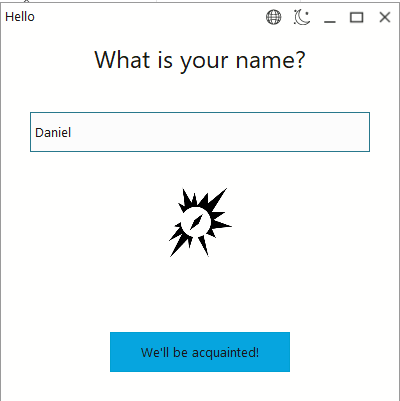
\includegraphics[width=0.5\linewidth]{test1}}
\center{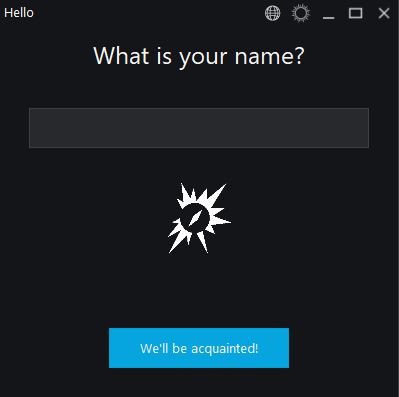
\includegraphics[width=0.5\linewidth]{test2}}
\caption{Cмена темы}
\label{theme:image}
\end{figure}

Функция: смена языка.

Условия: нажата кнопка смены языка.

Входные данные: данные для русского языка, данные для английского языка.

Результат: изменение текста окна и внутренних элементов (рисунок \ref{lang:image}).

\begin{figure}[H] % H - рисунок обязательно здесь, или переносится, оставляя пустоту
	\center{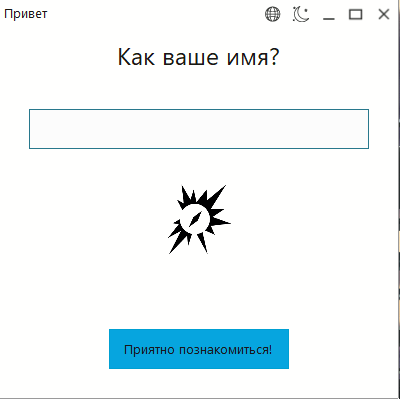
\includegraphics[width=0.5\linewidth]{test3}}
	\center{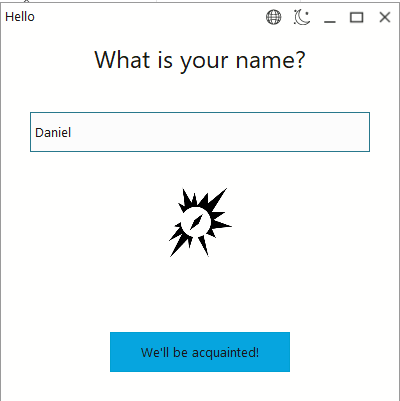
\includegraphics[width=0.5\linewidth]{test1}}
	\caption{Cмена языка}
	\label{lang:image}
\end{figure}

Функция: всплывающее окно.

Условия: введен текст, нажата кнопка подтверждения.

Входные данные: текст из поля ввода.

Результат: появление окна приветствия (рисунок \ref{msg:image}).

\begin{figure}[H] % H - рисунок обязательно здесь, или переносится, оставляя пустоту
	\center{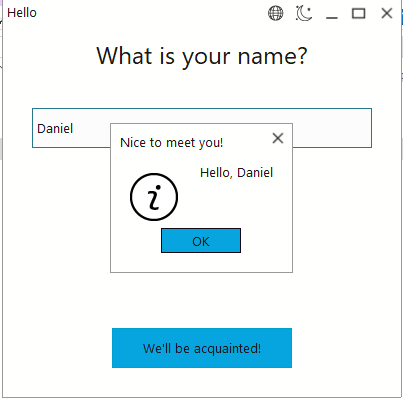
\includegraphics[width=0.8\linewidth]{test4}}
	\caption{Всплывающее окно}
	\label{msg:image}
\end{figure}

Функция: окно подтверждения.

Условия: нажата кнопка выхода из приложения.

Входные данные: событие нажатия кнопки мыши на кнопку закрытия.

Результат: появление окна закрытия (рисунок \ref{msg-y-n:image}).

\begin{figure}[H] % H - рисунок обязательно здесь, или переносится, оставляя пустоту
	\center{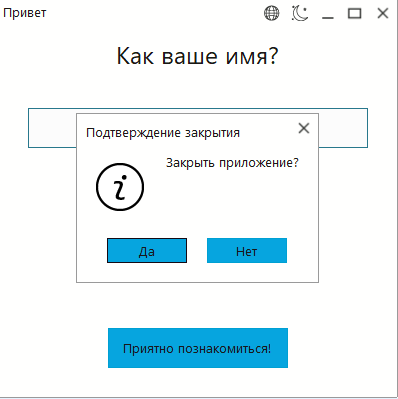
\includegraphics[width=0.8\linewidth]{test15}}
	\caption{Окно подтверждения закрытия}
	\label{msg-y-n:image}
\end{figure}

Функция: подсказка.

Условия: наведение курсора мыши на иконку кнопки.

Входные данные: положение курсора, обработчик события подсказки.

Результат: появление подсказки под кнопкой (рисунок \ref{tip:image}).

\begin{figure}[H] % H - рисунок обязательно здесь, или переносится, оставляя пустоту
	\center{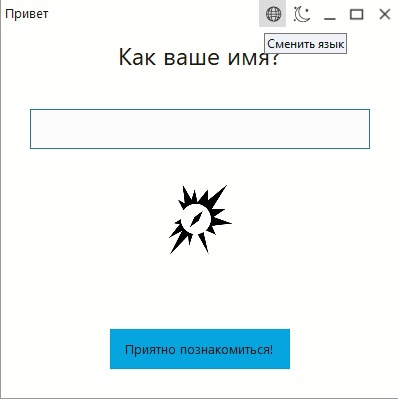
\includegraphics[width=0.8\linewidth]{test14}}
	\caption{Подсказка}
	\label{tip:image}
\end{figure}

Функция: развернуть окно во весь экран.

Условия: нажата кнопка "<Развернуть">.

Входные данные: размер экрана, обработчик события кнопки "<Развернуть">, состояние окна.

Результат: окно развернулось на полный экран, изменился размер внутренних элементов окна. (рисунок \ref{fullscreen:image}).

\begin{figure}[H] % H - рисунок обязательно здесь, или переносится, оставляя пустоту
	\center{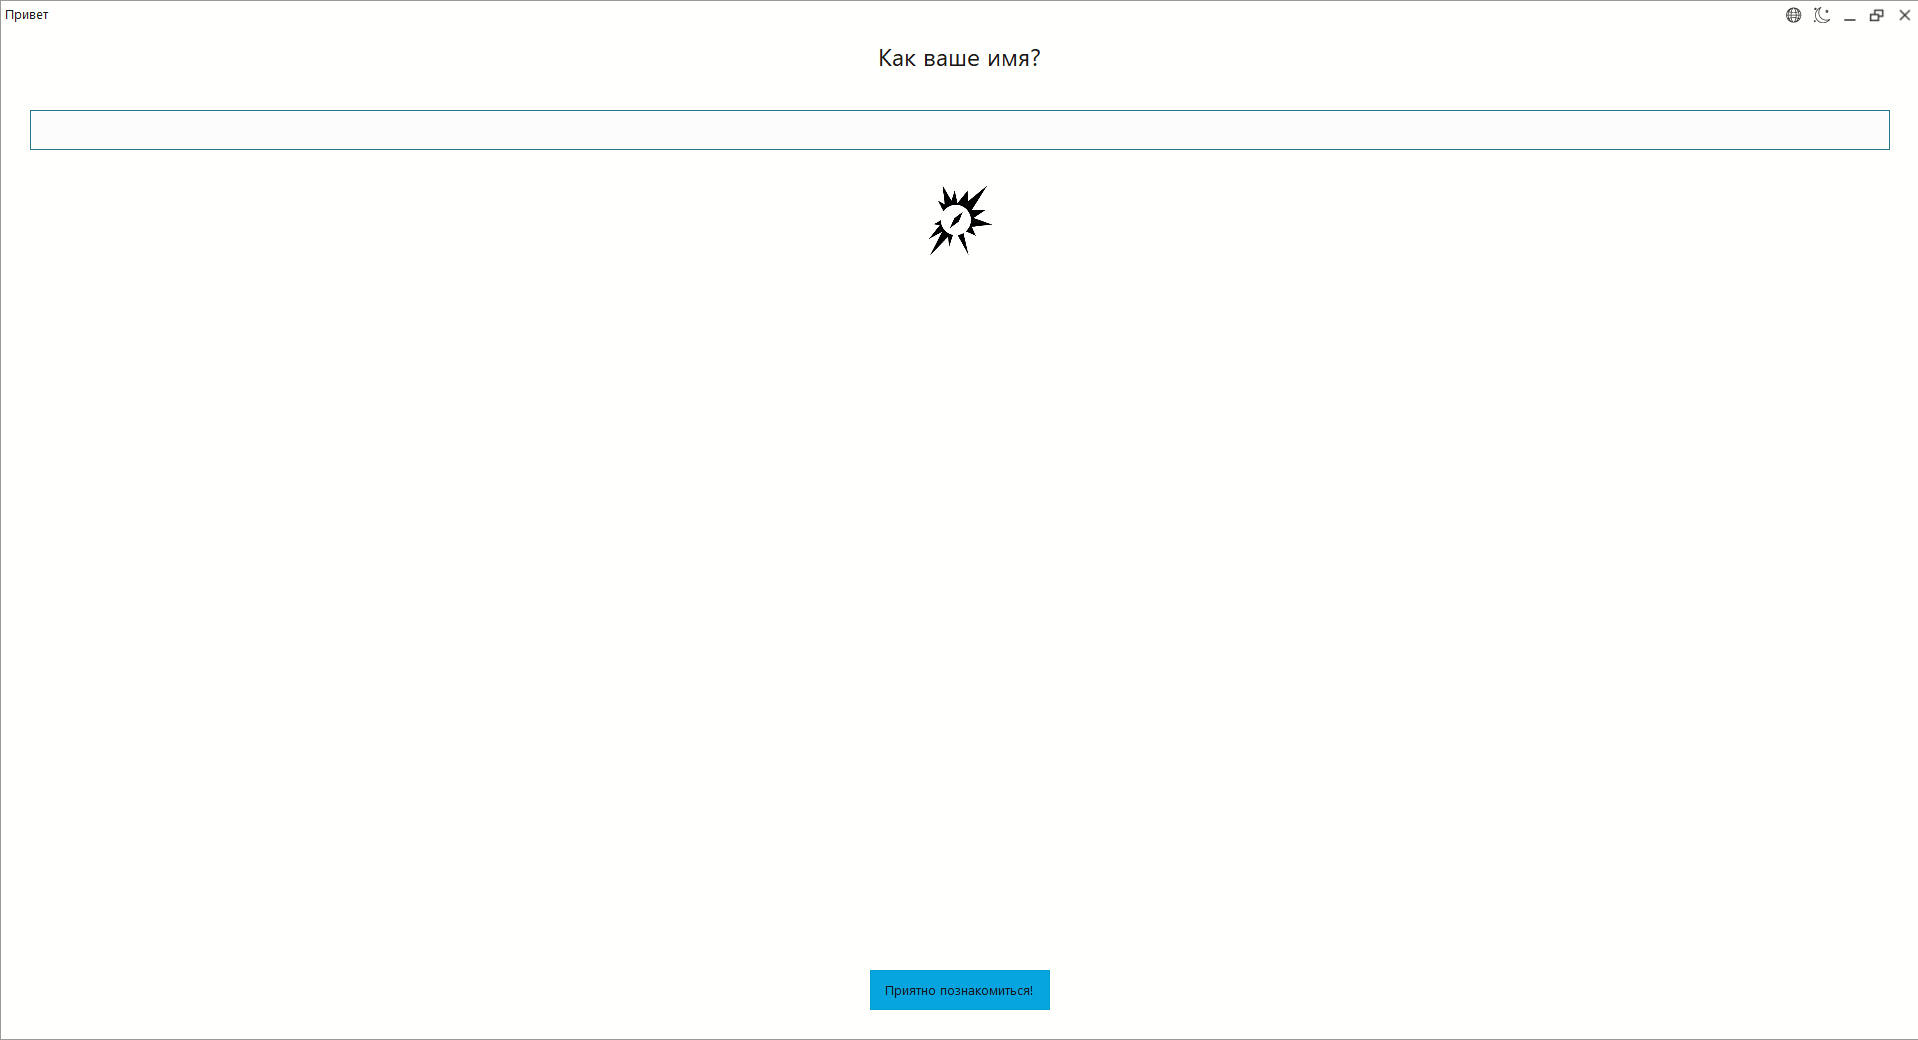
\includegraphics[width=0.8\linewidth]{test16}}
	\caption{Приложение, развернутое на полный экран}
	\label{fullscreen:image}
\end{figure}

Функция: ползунок.

Условия: изменено положение ползунка.

Входные данные: позиция ползунка, обработчик события ползунка.

Результат: на экране появилась координата х, в случае изменения положения горизонтального ползунка, и координата y при изменении положения вертикального ползунка.
. (рисунок \ref{scroll:image}).

\begin{figure}[H] % H - рисунок обязательно здесь, или переносится, оставляя пустоту
	\center{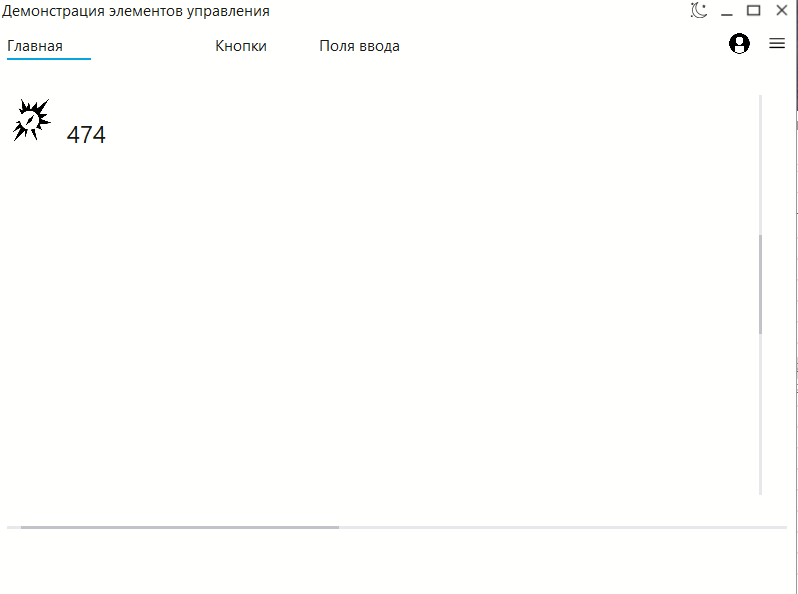
\includegraphics[width=0.8\linewidth]{test7}}
	\caption{Ползунок}
	\label{scroll:image}
\end{figure}

Функция: поле для ввода.

Условия: в поле для ввода введен текст.

Входные данные: фокус поля для ввода, обработчик события клавиатуры.

Результат: на экране появился текст.
. (рисунок \ref{input:image}).

\begin{figure}[H] % H - рисунок обязательно здесь, или переносится, оставляя пустоту
	\center{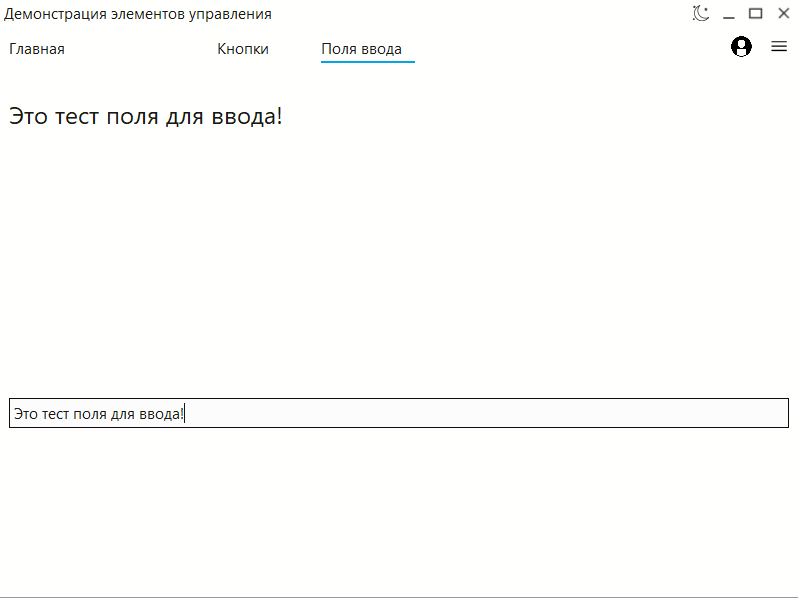
\includegraphics[width=0.8\linewidth]{test17}}
	\caption{Поле для ввода}
	\label{input:image}
\end{figure}

Функция: нажатие кнопки.

Условия: нажатие кнопки мыши на кнопку.

Входные данные: событие нажатия кнопки мыши на кнопку, нажатая кнопка.

Результат: появилось текстовое сообщение о том какая кнопка нажата. (рисунок \ref{button:image}).

\begin{figure}[H] % H - рисунок обязательно здесь, или переносится, оставляя пустоту
	\center{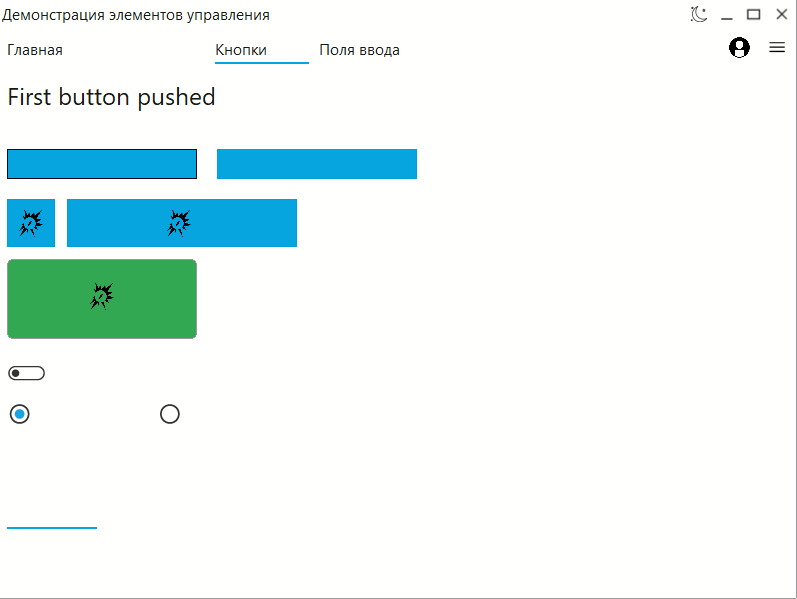
\includegraphics[width=0.8\linewidth]{test5}}
	\caption{Нажатие кнопки}
	\label{button:image}
\end{figure}

Функция: нажатие переключателя.

Условия: нажатие кнопки мыши на переключатель.

Входные данные: событие нажатия кнопки мыши на переключатель, нажатый переключатель.

Результат: появилось текстовое сообщение о том, что нажат переключатель. (рисунок \ref{switcher:image}).

\begin{figure}[H] % H - рисунок обязательно здесь, или переносится, оставляя пустоту
	\center{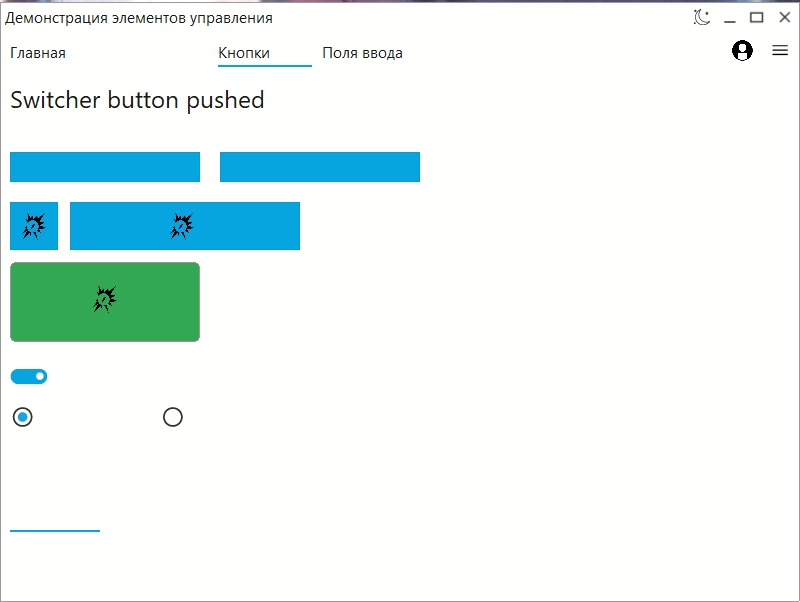
\includegraphics[width=0.8\linewidth]{test10}}
	\caption{Нажатие переключателя}
	\label{switcher:image}
\end{figure}

Функция: радиокнопка.

Условия: нажатие кнопки мыши на радиокнопку.

Входные данные: событие нажатия кнопки мыши на радиокнопку, нажатая радиокнопка.

Результат: появилось текстовое сообщение о том, что нажата радиокнопка. (рисунок \ref{radio:image}).

\begin{figure}[H] % H - рисунок обязательно здесь, или переносится, оставляя пустоту
	\center{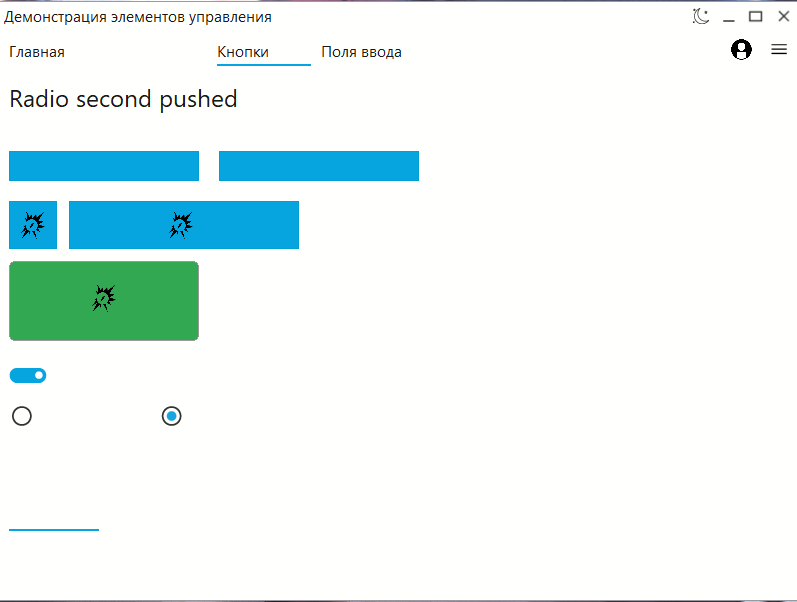
\includegraphics[width=0.8\linewidth]{test11}}
	\caption{Нажатие радиокнопки}
	\label{radio:image}
\end{figure}

Функция: смена страницы.

Условия: нажатие кнопки мыши на страницу.

Входные данные: событие нажатия кнопки мыши на страницу, нажатая страница.

Результат: появилось текстовое сообщение о том, что нажата страница. (рисунок \ref{sheet:image}).

\begin{figure}[H] % H - рисунок обязательно здесь, или переносится, оставляя пустоту
	\center{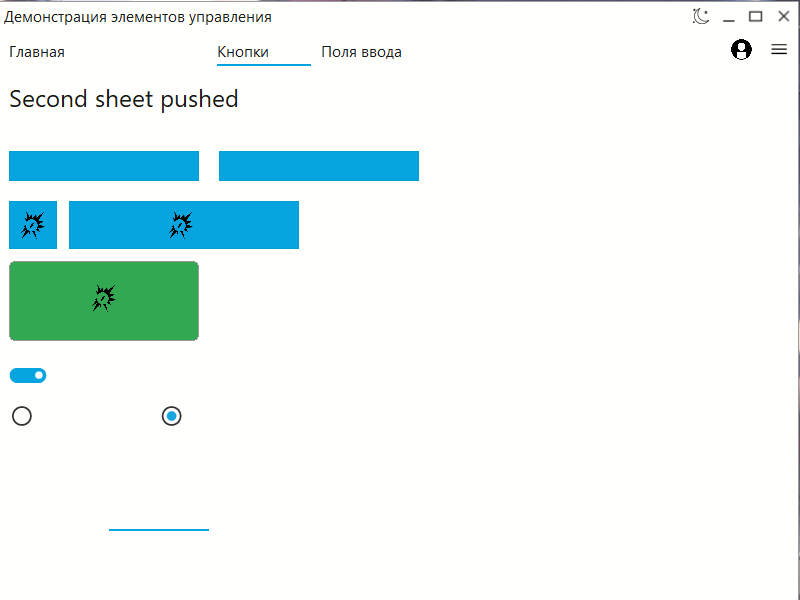
\includegraphics[width=0.8\linewidth]{test12}}
	\caption{Кнопка смены страницы}
	\label{sheet:image}
\end{figure}

Функция: ползунок настройки и полоса прогресса.

Условия: передвинут ползунок настройки.

Входные данные: положение ползунка настроек, обработчик событий.

Результат: при изменении положения ползунка настроек заполняется полоса прогресса. (рисунок \ref{slider:image}).

\begin{figure}[H] % H - рисунок обязательно здесь, или переносится, оставляя пустоту
	\center{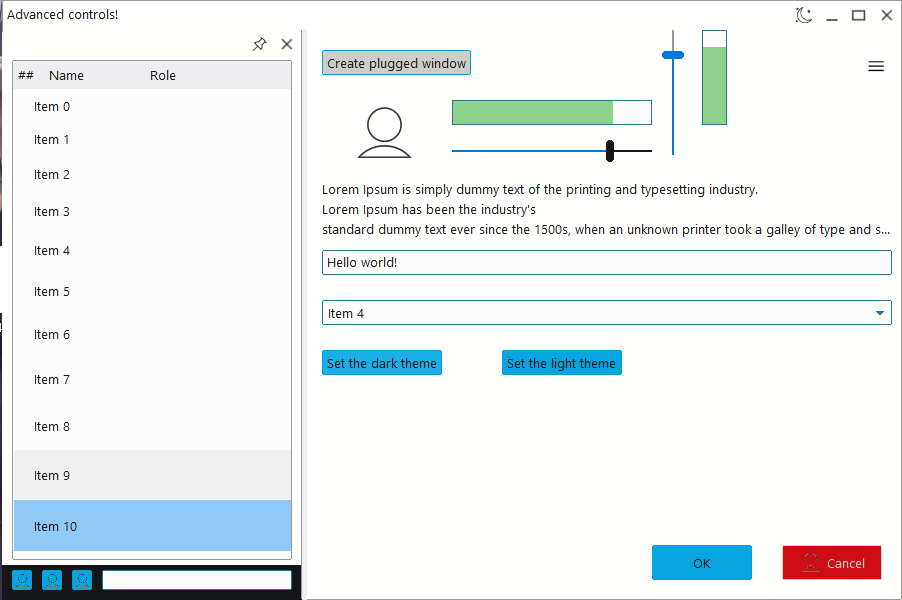
\includegraphics[width=0.8\linewidth]{test13}}
	\caption{Ползунок настройки и полоса прогресса}
	\label{slider:image}
\end{figure}

Функция: выпадающий список.

Условия: нажатие кнопки мыши на выпадающий список.

Входные данные: нажатие кнопки мыши на выпадающий список, обработчик события списка.

Результат: Раскрытие выпадающего списка. (рисунок \ref{list:image}).

\begin{figure}[H] % H - рисунок обязательно здесь, или переносится, оставляя пустоту
	\center{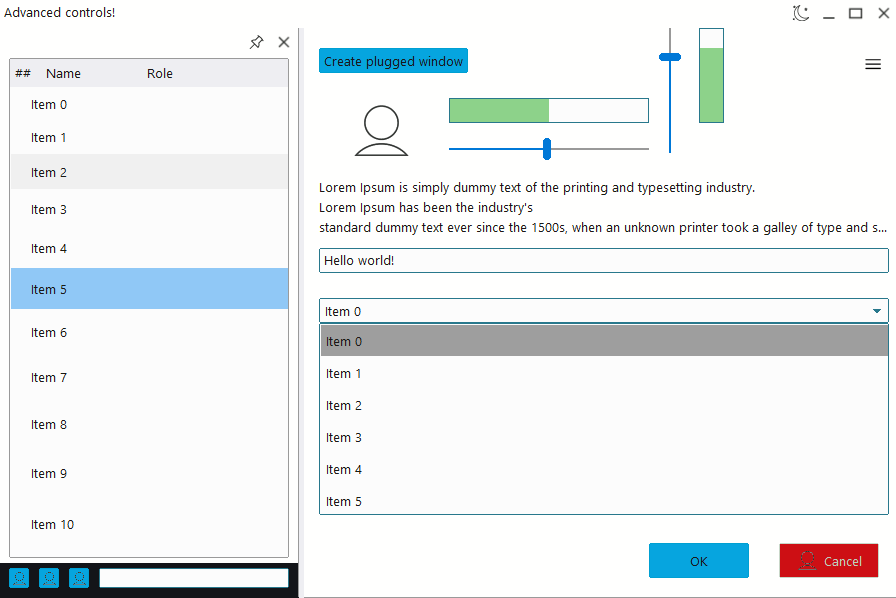
\includegraphics[width=0.8\linewidth]{test8}}
	\caption{Cписок}
	\label{list:image}
\end{figure}

Функция: Меню.

Условия: нажата кнопка настроек.

Входные данные: нажатие кнопки мыши на кнопку настроек, обработчик меню настроек.

Результат: на экране появилось меню. (рисунок \ref{menu:image}).

\begin{figure}[H] % H - рисунок обязательно здесь, или переносится, оставляя пустоту
	\center{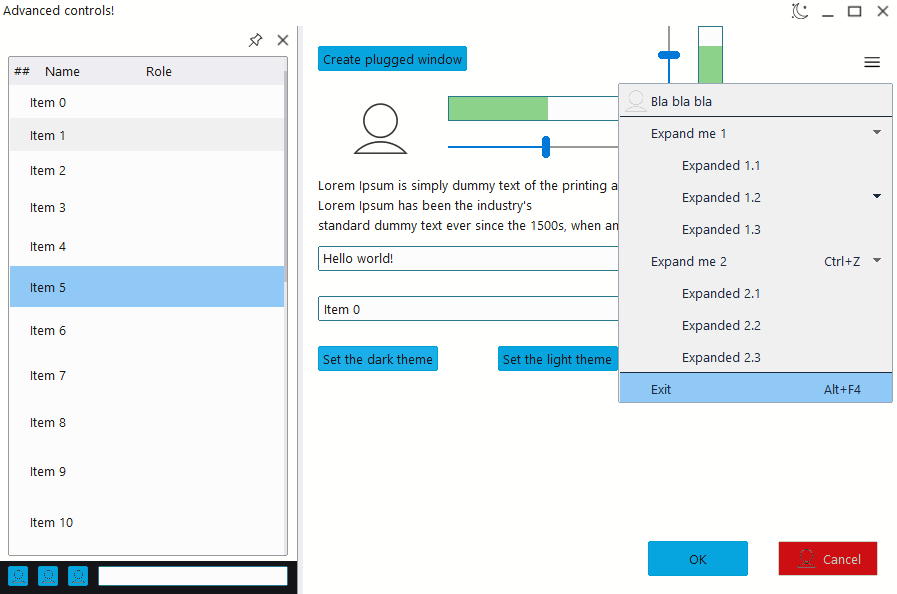
\includegraphics[width=0.8\linewidth]{test9}}
	\caption{Меню настроек}
	\label{menu:image}
\end{figure}

Функция: открепление окна.

Условия: нажатие кнопки мыши на кнопку открепления окна.

Входные данные: нажатие кнопки мыши на кнопку открепления окна, позиция окна, состояние окна, обработчик события.

Результат: появилось открепленное окно, которое можно двигать по экрану. (рисунок \ref{pin:image}).

\begin{figure}[H] % H - рисунок обязательно здесь, или переносится, оставляя пустоту
	\center{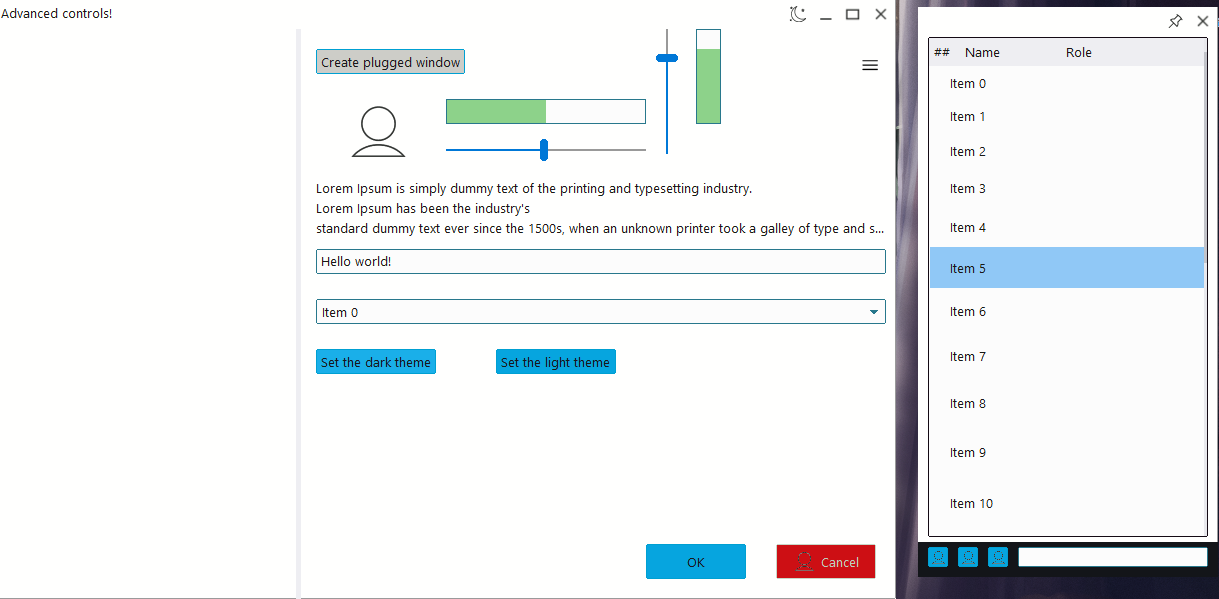
\includegraphics[width=0.8\linewidth]{test6}}
	\caption{Открепление окна}
	\label{pin:image}
\end{figure}